% \pagebreak[4]
% \hspace*{1cm}
% \pagebreak[4]
% \hspace*{1cm}
% \pagebreak[4]

\chapter{Background}
\ifpdf
    \graphicspath{{Chapter1/Chapter1Figs/PNG/}{Chapter1/Chapter1Figs/PDF/}{Chapter1/Chapter1Figs/}}
\else
    \graphicspath{{Chapter1/Chapter1Figs/EPS/}{Chapter1/Chapter1Figs/}}
\fi

\section{Software Engineering}
There is an inherent scale and complexity existing in modern software. Contributors to this complexity include the accession of cheap and powerful hardware, software features such as graphical user interfaces and other layers of conceptualization and abstraction that didn't exist in earlier programming languages. The size of software has increased. It's not uncommon for a system to contain millions of lines of code and beyond - Microsoft Windows operating system Vista reputedly has over 50 million. This modern-age complexity makes developing and maintaining software a tricky business. As stated by Lanza,

\begin{quote}
Designing large applications is difficult because of the intrinsic complexity of the modelled domains. To this intrinsic complexity, another incidental factor is added, which comes from business processes, organizational issues, human and other external factors \citep[pg.~1]{lanza06}.
\end{quote} 

So what can we do to overcome the barriers of working with large and complicated systems? The modern solutions to these problems involve iterative development methodologies, unit testing, application of design patterns and principles, and refactoring. There are two tools which have been proven to scale up and be successful when dealing with large legacy systems, and these are metrics and visualization \citep{lanza06}. 

\subsection{Current Software Engineering Practices}
A number of software engineering practices have been devised to combat the issues of scale and complexity in software development. In an effort to replicate the practices of traditional engineering disciplines, these practices include measurement, analysis and interpretation of results.

\subsubsection{Development Methodologies}
A number of development methodologies have been devised to effectively plan and control the software development process. The waterfall model of development proposed producing requirements analysis and detailed design documents up-front. This was refined in the spiral model which combined iterative development with the structured design process of the waterfall model to allow a more flexible approach. Finally, agile development methodologies (introduced by the Agile Manifesto \citep{beck01}) were devised which promote a more adaptive and flexible approach to design and development. Responsibility driven design is a technique which focuses on the contract between a client and a server. Peer code reviews, where a developer reviews code written by someone else, are also now promoted as good practice.  Development methodologies and their process metrics allow the state and transition of a project to be measured.  


\subsubsection{Automated Unit Testing and Continuous Integration}

Automated unit testing tools such as jUnit\footnote{\url{http://www.junit.org/}} and nUnit\footnote{\url{http://www.nunit.org/}} execute suites of tests written by developers in the target language, which test that each unit of code is behaving as expected. One practice is to test contracts of an interface. Unit testing is a key feature of Agile methodologies such as Test Driven Development, where it is expected that a test for a given module of code will be written before the module itself is produced. The module is not considered complete before the unit test has passed. This practice has been shown in empirical studies to produce a significant increase (more than double) in code quality than products developed without using Test Driven Development \citep{bhat06}. Through automated unit testing we are able to measure software fault density, location and severity. We can also measure the quality and adequacy of the testing. Continuous integration.

\subsubsection{Object-Oriented Design Principles}

Over the years, a number of important software engineering principles and techniques have been defined.  Concepts such as separation of concerns, abstraction and encapsulation are important techniques in an object-oriented programming design.  In addition to these general principles, more specific and definable principles have been developed. These principles primarily assist to decouple software modules, and therefore make code bases easier to maintain, understand and extend.

Inheritance is a fundamental mechanism in the object-oriented paradigm, but  ``can be a tricky technique to get correct - it is often one of the most abused features in object-oriented languages'' \citep{pugh06}. With implementation inheritance, the derived class is tightly coupled with the base class. If you alter the base class, this can have unintended consequences for its derived types - this is known as  the fragile base class problem, as described by \citet{mikhajlov98}. It is also possible for the derived class to break the contracts promised by the base class. In ``Holub on Design Patterns'', \citet{holub04} recommends that you avoid implementation inheritance whenever possible and instead design to an interface.

Design by Contract\texttrademark by \citet{meyer92} is centred around the premise that successful use of an interface requires a standard contract between a caller and an implementer of an interface. This contract is a formalization of the obligations and benefits between a client and supplier code module.  

The Law of Demeter states that each program unit should have only limited knowledge about other units. An object should make as little assumptions as possible about the structure or properties of any other object \citep{lieberherr96}.

Robert Martin's book ``Agile Software Development, Principles, Patterns, and Practices'' popularized the five SOLID principles of programming.  The first principle in this set is the Single Responsibility Principle - every object should have only a single responsibility, and that responsibility should be entirely encapsulated by the class \citep{martin02}. This principle is heavily used in responsibility driven design methods. The Open/Closed principle states that ``software entities (classes, modules, functions, etc.) should be open for extension, but closed for modification'' \citep{meyer88}. In other words, software should be designed so that new functionality may be added with minimal changes. The Liskov Substitution Principle says that if a program module inherits a base class, then the reference to the base class should be able to be replaced with a derived class without changing the programs behaviour. Derived types must be completely substitutable for their base types \citep{liskov87}. In the Interface Segregation Principle, clients should not be forced to implement interfaces they don't use. Instead of one large interface, it is preferred to use many small interfaces based on groups of methods \citep{martin96isp}. The final principle in this set is the Dependency Inversion Principle - this is form of decoupling where the tradition dependency model is reversed. A layer of abstraction should be placed between high level and low level modules and each module should depend upon this abstraction, rather than on each other \citep{martin96dip}. Dependency injection is one method of following this principle. 

We can measure violations of rules against a defined set of design principles \citep{marinescu04}.

%detect presence or absence of principles. Measure how well they are applied

\subsubsection{Object-Oriented Design Heuristics and Patterns}

The object-oriented design principles are supported by patterns which provide solutions to common software engineering problems. The quintessential guide for design patterns ``Design Patterns: Elements of Reusable Object-Oriented Software'', written by the Gang of Four, presented 23 patterns which were divided into creational, behavioural and structural areas \citep{gamma94}. The book focused on patterns designed for C++. It has been demonstrated by \citet{norvig} that 16 of these patterns are simplified or eliminated by direct language support in Lisp or Dylan. The original set of patterns have since be expanded. %(example?). 

Design patterns can be classified into further subtypes. There are service patterns, integration patterns, enterprise patterns, analysis patterns, anti-patterns and others. Integration patterns answer questions about how multiple applications can be integrated to work together and to exchange information \citep{fowler03}. These patterns are incorporated in open-source frameworks Mule, Apache camel and Spring Integration. Service patterns are for designing programs that can be interacted with through well-defined message exchanges. Analysis patterns highlight commonalities in domain model structure. Anti-patterns are patterns that are commonly used but may be ineffective or damaging.

%Patterns that describe best practices in re-engineering legacy systems \cite{demeyer03, feathers04}. 

While a design pattern creates a solution for a specific problem, heuristics are general guidelines in design. Design heuristics presented by \citet{riel96} are guidelines intended for the detection of good/bad object-oriented design. It is interesting to note that design patterns can violate heuristics. For example, the command pattern, in which an object is used to represent all information needed to call a method at a later time violates Riel's heuristic 3.9 - do not turn an operation into a class. %(Lang, C. et al)

We can measure and detect the presence of good design patterns or anti-patterns indicating a need for refactoring.

\subsubsection{Refactoring}

As described by \citeauthor{fowler99} in the 1999 classic refactoring reference \textit{Refactoring: Improving the Design of Existing Code};

\begin{quote}
Refactoring is the process of changing a software system in such a way that it does not alter the external behaviour of the code yet improves its internal structure \citep[pg.~xvi]{fowler99}.
\end{quote} 

In other words, refactoring is altering the underlying software design without changing the functionality. This is at odds with earlier styles of software development where refactoring was avoided through the fear of unintended consequences. Refactoring is typically with a goal of allowing greater understandability and extensibility - paving the way for future modifications of the code. The key benefits of refactoring are to simplify maintenance and to provide a better platform for ongoing future development. 

Refactoring can be described is an ongoing refinement process, which should be evoked as software evolves over time. \citeauthor{opdyke92}, who in his 1992 phd thesis published the first reference to refactoring objected-oriented code, states that;

\begin{quote}
Design is hard. The design of reusable software is especially hard. Reusable software usually is
the result of many design iterations. Some of these iterations occur after the software has been
reused, and the resulting changes affect not only the design of the reusable software, but also
the design of other software that is using it. Making software easier to change makes subsequent
design iterations easier, and makes the software more reusable~\citep{opdyke92}.
\end{quote} 

Fowler's refactoring techniques can be grouped into areas of improving data organisations, simplifying conditional expressions, improving abstraction, and breaking code into more logical pieces amongst others. Examples of  techniques can be found on Martin Fowler's website\footnote{\url{http://martinfowler.com/refactoring/catalog/index.html}}.

% (Other possible citation for refactoring: Refactoring to patterns, Joshua Kerievsky).

Code smells are certain patterns or structures within software. The presence of a bad code smell indicates there is a possibility of a design flaw and the code would benefit from being restructured through refactoring. The term ``code smell'' was coined by Kent Beck and popularised in \cite{fowler99}, where it was suggested they could be used when trying to determine where and how much code to refactor. There is a degree of intuition required in identifying code smells, ``you have to develop your own sense of how many instance variables are too many instance variables and how many lines of code in a method are too many lines''~\citep[pg.~75]{fowler99}. 

Code smells may be generally grouped into structural problems of size (long methods, large classes, too many parameters), relationship (message chains, inappropriate intimacy) and inheritance (refused bequest, parallel inheritance hierarchies).

In order to ensure the code's external behaviour is not modified and bugs are not introduced during the refactoring processing, the use of automated unit testing is an important prerequisite. 

\subsection{Software Analysis}

With the modern approaches to software design and development created to help implement complex systems - such as agile development processes, automated unit testing, application of design patterns, principles and heuristics and continuous refactoring - we still require a way of accurately measuring the quality of the software.  Furthermore, we need a way of predicting or analysing which parts of the software system require change.

\subsubsection{Dynamic and Static Software Analysis Tools}

Automated dynamic or static software analysis tools provide a variety of ways to measure a system. 

Dynamic software analysis involves the collection of data during the execution of the system. This kind of analysis has several different motivations. Runtime debuggers allow you to step through a running process. Code profilers allow you to find performance hotspots. Code coverage tools such as Cobertura\footnote{\url{http://cobertura.sourceforge.net/index.html}} and NCover\footnote{\url{http://www.ncover.com/}} measure the amount the amount of software that has been executed. This can be very useful for determining software testing thoroughness, where the efficiency of the tests are estimated by measuring the amount of actual code executed during a test run. Memory analysis tools such as the Eclipse Memory Analyzer\footnote{\url{http://www.eclipse.org/mat/}} track the memory usage of the software in order to locate leaks and reduce memory consumption.  DTrace\footnote{\url{http://dtrace.org/blogs/about/}} is an instruction tracing tool that creates a record of what happens as the code is executed. This is done by dynamically patching live running instructions with instrumentation code. DTrace is an example of a performance analysis tool, used to identify bottlenecks and allow fine-tuning of software for better performance.

The problem with dynamic analysis tools is they are used late in the development cycle. It is generally considered to be more costly to fix a defect the further along in the development cycle it is found. Static analysis deals with the structure and development of the source code and may be performed much earlier in the development cycle. This analysis includes calculating source-code metrics, using defined patterns to detect potential bugs, and finding instances where coding conventions and rules were broken. Potentially vulnerable or defect-prone areas of code may be located. Some types of static analysis are code reviews, and dependency, complexity and trend analysis. Example tools using static analysis are Checkstyle\footnote{\url{http://checkstyle.sourceforge.net/}}, PMD\footnote{\url{http://pmd.sourceforge.net/pmd-5.0.0/}} and FindBugs\footnote{\url{http://findbugs.sourceforge.net/}}. An advantage of static code analysis is that defects may be found in parts of code not executed during normal program operation such as error handling routines, or issues involving memory corruption or leaked system resources. %find reference for more costly to fix a defect the further along in the development cycle

\subsubsection{Software Metrics}

According to \citet{fenton98}, ``measurement is the process by which numbers or symbols are assigned to attributes of entities in the real world, in such a way as to describe them according to clearly defined rules''.  Measurement is important in engineering disciplines, and so the software engineering community has defined various metrics of software with the purpose of producing quantifiable measurements. Software metrics are measurements of specific elements of software entities. They are used to summarise software and detect outliers in large volumes of data. These measurements may then be used for a variety of reasons including being able to make informed decisions about the software, improve its overall quality and determine the progression of specific projects.``Without such measures for managing software, it is difficult for any organization to understand whether it is successful, and it is difficult to resist frequent changes of strategy.'' \citep{grady92}.

Metrics based on software source code may be grouped into various categories such as:

\begin{itemize}
	\item \textit{Size} - Measuring size of counting attributes. Examples of this kind of metric are LOC, SLOC, KLOC or Halstead software science.
	\item \textit{Complexity} - Measuring the complexity of flow and data control structures such as cyclomatic complexity and NPATH.
	\item \textit{Object-oriented metrics} - Metrics computing complexity for object oriented languages. The most common example of this is the Chidamber and Kemerer suite.
	\item \textit{Quality} - Metrics calculating intrinsic software quality. Examples include defect density and MTTF.
	\item \textit{Process} - Measuring the effectiveness of the software process. Examples include defects reported by end-users, human effort and calendar time expended.
\end{itemize}

Comprehensive details on various software metrics and their calculations and usages may be found in \citet{fenton98} and \citet{hendersonsellers95}.

There are some challenges in the usage of metrics for measuring software quality. In practice there is not widespread adoption of metric use. Secondly, there is no standardisation of metric calculations and this leads to different results from different tools.

There have been a wide variety of metrics defined but selecting a set of metrics has to be based on the purpose of measuring. In other words we need to collect metrics that answer the questions we are posing about the software.

\subsubsection{Software Visualisation}

The modern world is awash with information leaving many people overwhelmed with information overload.  Information visualisation is a method for gaining insight into data through graphical interaction and exploration. Accurate and effective visualisation of data is important and necessary in the modern world because increasingly ``there are many situations in which data is available, sometimes in very large quantities, and where some human insight into that data is required.''~\citep{spence07}. An example of a well known information visualisation - the London Underground tube map is found at Fig. \ref{fig:londontube}.

\begin{figure}[h!]
  	 \centering
   	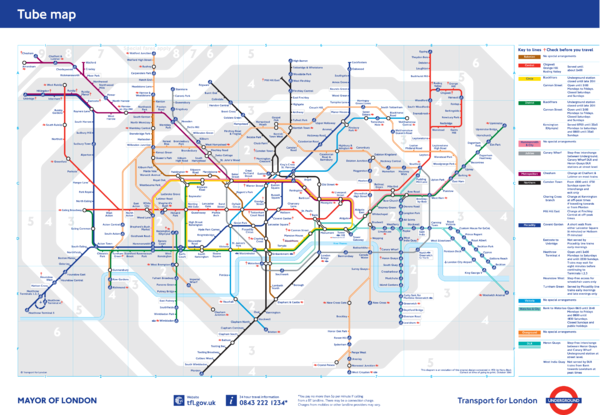
\includegraphics[width=140mm]{londontube.png}
  	\caption{London Underground Tube Map}
	\label{fig:londontube}
\end{figure}

%more citations for information visualisation \cite{ware04, ware08} software vis \cite{lanza06} 

Software visualisations are a subset of a larger group of information visualisations and are visual representations of software with the purpose of supporting a greater understanding of a software system. ``Software visualization is the use of the crafts of typography, graphic design, animation and cinematography with modern human-computer interaction and computer graphics technology to facilitate both the human understanding and effective use of computer software'' \citep{price93}. A popular example of a software visualization is a UML (Unified Modeling Language) diagram. %UML diagram not good at evolving software systems.

There are a variety of factors to consider when visualising software; many variables, huge data volumes and a need for understanding the data in context. It is necessary to be alerted the presence of outliers in data sets. %Skewed data

%(Review types of software visualisation, popular tools or frameworks, and research relating to these).
%Types of software visualisation may include algorithm animation, software architecture, software evolution, data mining and visual analytics. 
%What are the issues with current visualisation tools? User studies? 
%How can we tailor the visualisation to best fit the task?
%Structure charts. Ternary diagrams. Treemaps.
%What tasks do users have (fnd where X is declared, who calls Y, . . .) IDE can help. Where am I? what method am I looking at? 

In the visualisation of software metrics, we need to deal with multivariate data. How many variables can we map in a visualisation? At what point when increasing the number of variables does it become counter-productive? Multivariate data can be modelled with charts histograms or scatterplots, but something more powerful is needed in the object-oriented paradigm. Treemaps are a popular technique for displaying software visualisation because they are effective at showing hierarchical relationships such as inheritance in object-oriented software. See Fig. \ref{fig:treemap}.

\begin{figure} [h!]
  	 \centering
   	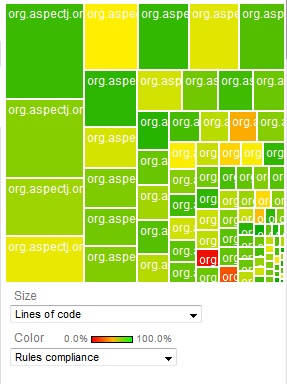
\includegraphics[width=60mm]{treemap.png}
  	\caption{Aspectj Treemap}
	\label{fig:treemap}
\end{figure}


Some studies have looked at the value of 3D visualisations \citep[such as][]{irwin03}, where 3D virtual worlds for visualising software metrics were explored. \citet{mendes11} used building block metaphors to create an interactive LEGO application. In software visualisation, it is necessary to smoothly transition from one visualisation/mapping to another in sequence of activities. \citet{harward10} described code colouring, used to augment development environments within an existing IDE interface. These in situ visualisations may provide more context for users than separate window/application visualisations. It is possible to create an ambient visualisation using alternate senses via sound, odour, or vibration. \citet{murphyhill10} proposed a novel smell detector called Stench Blossom, that provided an interactive ambient visualization designed to first give programmers a high-level overview of the smells in their code. %mouse feedback

%Other citations \cite{lorenz94, hendersonsellers95}

\section{Tag Clouds}

Tag clouds are a common example of information visualisation and are used to embody text - words, two-word phrases and symbols. These items are grouped together to form a visual representation of the data.  Each element of the visualisation is referred to as a tag - this may be website keywords which are hyperlinked to related resources. The frequency of a word (and therefore assumed importance) is highlighted by the font size or colour.  This makes the most important and prominent keywords easy to quickly identify as well as showing the relative importance of keywords. They can be displayed in a variety of layouts, most commonly alphabetically (see Fig. \ref{fig:tagcrowd} for a typical example).

\begin{figure}[h!]
   \centering
   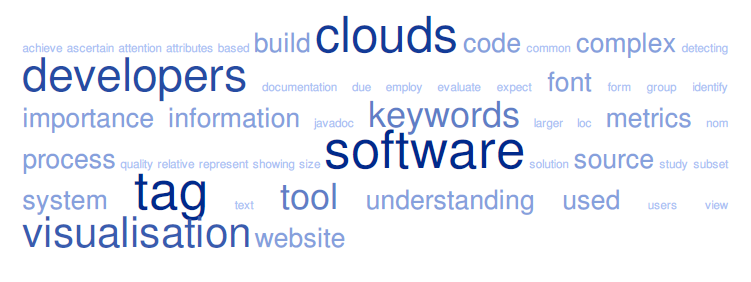
\includegraphics[width=140mm]{tagcrowd.png}
  \caption{Tag cloud created by TagCrowd}
  \label{fig:tagcrowd}
\end{figure}

As an effective visualisation, tag clouds are noted to contain some drawbacks. When rendering a large volume of data, increasing the cloud size decreases the ability to draw any meaning from the text. There are inconsistencies in the distribution of font sizes and tag weights.  Finally, tag clouds provide limited interaction with the user.

%If a user can't predict what it means for a tag be a certain size every time a cloud is viewed, then its size has little meaning for the user \citep{hoffman06}.

\subsection{History}

An early example of a weighted list of keywords can be found in Douglas Coupland's 1995 novel Microserfs. In this novel, a computer algorithm selects random phrases from an electronic diary creating a set of ``subconcious files''. In 2002 Jim Flanagan created a Perl module (Search Referral Zeitgeist), which generated a graphic of website referrers. Based on this implementation, photosharing site Flickr\footnote{\url{http://www.flickr.com}}, founded in 2004, created a ``tag cloud'' visualisation showing tag popularity through font size. Tag clouds then started appearing as a navigation aid on Web 2.0 websites such as Del.iocio.us\footnote{Now known as \url{http://www.delicious.com/}}.

The tag cloud was further adapted in 2006 by TagCrowd\footnote{\url{http://tagcrowd.com/}} for visualizing word frequency in text, and then popularised by Wordle\footnote{\url{http://wordle.net/}} \citep{feinberg10}. Wordle showed tag clouds had the ability to be aesthetically pleasing (see Fig. \ref{fig:wordle}).

\begin{figure}[h!]
   	\centering
   	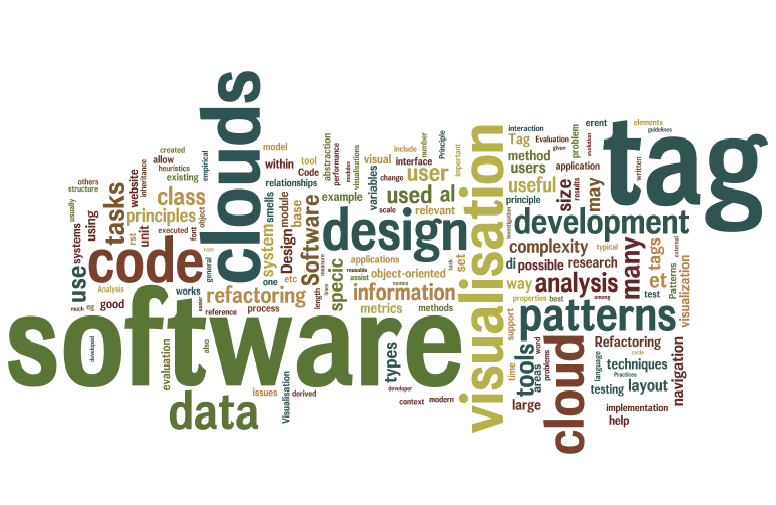
\includegraphics[width=140mm]{thesistagcloud.png}
  	\caption{Tag cloud created by Wordle}
	\label{fig:wordle}	
\end{figure}

\subsection{Related Work - Extensions and Evaluations}

There has been a spate of research in recent years evaluating tag cloud usage. \citet{rivadeneira07} conducted an early empirical tag cloud evaluation, and proposed a set of user tasks supported by tag clouds. These include searching, browsing, impression forming and recognition/matching. Font size has been discovered to have a strong effect on user perception \citep[]{rivadeneira07, bateman08, halvey07}, although \citet{bateman08} suggested this effect is influenced by other visual properties. Evaluation of eye-tracking data by \citet{lohmann09} supports this suggestion.

It has been noted that tags in the upper left quadrant of a tag cloud are found more quickly \citep{bateman08} and are better recalled \citep{rivadeneira07}. Analysis of eye-tracking data has shown the upper left quadrant of a tag cloud receives the most attention \citep[][]{lohmann09, schrammel09b}. 

Studies \citep[such as][]{halvey07, bateman08} have suggested users `scan' tag clouds rather than read them.  Research considering visual exploration strategies of tag clouds and recorded gaze data has supported this finding \citep[][]{lohmann09, schrammel09b}. In their extensive study of visual perception of tag clouds, \citet{schrammel09b} also found two types of user search strategy - chaotic and serial scanning. Users typically switched to serial scanning (performed in a characteristic zig-zag pattern), after a chaotic search pattern did not yield a result.

Using qualitative methods \citet{hearst08} investigated the motivations behind tag cloud usage. Results from their interviews indicated that users perceive a primary advantage of tag clouds as signallers of the social activity occurring within a system.

\citet{Oosterman10} conducted an empirical comparison of tag clouds and tables, and found evidence tables were faster and more accurate than tag clouds for specific element identification tasks. Other studies comparing tag clouds with lists \citep{halvey07, rivadeneira07, kuo07} found results indicated ordinary lists perform better than tag clouds for user search tasks, although \citet{kuo07} reported user satisfaction to be higher with tag clouds. \citet{sinclair08} found users preferred a traditional search interface for specific information retrieval tasks but the tag cloud was preferred where the information seeking was non-specific. They concluded tag clouds were worthwhile as a supplement to traditional interfaces rather than a replacement.

In the area of improvements to tag cloud construction and layout, \citet{kaser07} presented models and algorithms that leveraged work in typesetting and Electronic Design Automation. \citet{seifert08} proposed a family of novel algorithms to address issues of whitespace and overlapping tags. \citet{schrammel09} evaluated semantically clustered tag clouds for search and recall tasks. Results indicated that for specific search tasks, semantically clustered tag clouds could improve performance over random layouts, although not alphabetical layouts. \citet{halvey07} investigated tag presentation techniques in relation to properties. Results found users were able to more easily find tags in alphabetical order. 

Modified tag clouds have been proposed with various applications. \citet{Fujimara08} presented an algorithm for displaying large datasets in a tag cloud. \citet{Candan08} described a layout algorithm to display a hierarchy in a way that captures contextual relationships between tags and promotes navigation. \citet{Cui10} coupled a trend chart with word clouds to illustrate temporal content evolutions in a set of documents. \citet{dicaro08} investigated semantically informed navigation within a tag cloud. \citet{callegari10} evaluated tag cloud usage for image retrieval and \citet{lee10} integrated sparklines into tag clouds to convey trends between multiple tag clouds.

%Guidelines for designers of tag clouds \citet{bateman08}.

Much of this research may be drawn upon when considering the applications of tag clouds or other visualisations in the software engineering domain. For example, the identification of corresponding software engineering tasks to searching, browsing, impression forming and recognition/matching as classified by \citet{rivadeneira07}. The analysis of eye-tracking data showing user preference for the upper left quadrant of a visualisation \citep{lohmann09, schrammel09} is interesting, when reflecting that popularly used software diagrams such as UML, often contain the most relevant data towards the bottom (see Fig. \ref{fig:umldiagram}). The user `visual perception' element of visualisation in software seems to be poorly understood.

\begin{figure}[h!]
   \centering
   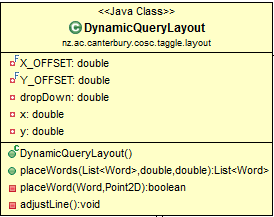
\includegraphics[width=60mm]{uml.png}
  \caption{UML Diagram}
  \label{fig:umldiagram}
\end{figure}


% ------------------------------------------------------------------------


%%% Local Variables: 
%%% mode: latex
%%% TeX-master: "../thesis"
%%% End: 
